% Copyright: 2016 Tim Weisenberger
% 2017 Modified by https://github.com/hubwoop
% Licence: cc by-nc

\documentclass[10pt,a4paper,landscape]{article}
\usepackage[left=0.65cm,right=0.65cm,top=1.85cm,bottom=0.75cm,landscape]{geometry} 
\usepackage{lastpage}
\usepackage{fancyhdr}
\usepackage{multicol}
\usepackage[ngerman]{babel}
\usepackage{ulem}
\usepackage{amsmath} 
\usepackage{amssymb}
\usepackage{setspace}
\usepackage{color}
\usepackage[dvipsnames]{xcolor}
\usepackage{titlesec}
\usepackage{tabularx}
\usepackage{array}
\usepackage{tikz}
\usepackage{ dsfont }
\usepackage{graphicx}
\usepackage{subcaption}
\usepackage{mathtools}
%\usepackage{lipsum} % dummy text
\newenvironment{Figure}
{\par\medskip\noindent\minipage{\linewidth}}
{\endminipage\par\medskip}

\DeclarePairedDelimiter\ceil{\lceil}{\rceil}
\DeclarePairedDelimiter\floor{\lfloor}{\rfloor}

% Header
\pagestyle{fancy}
\fancyhf{}
\fancyhead[L]{Formelsammlung - Mathematik I WS2016/2017}
\fancyhead[R]{Seite $\thepage$ von $\pageref{LastPage}$}

% Document
\setlength{\columnseprule}{0.5pt}
\setlength{\topskip}{\ht\strutbox} 
\setlength{\headheight}{0.1\baselineskip} 
\setcounter{secnumdepth}{4}
\newcolumntype{P}[1]{>{\centering\arraybackslash}p{#1}}
\newcolumntype{M}[1]{>{\centering\arraybackslash}m{#1}}

\titleformat{\paragraph}
{\normalfont\normalsize\bfseries}{\theparagraph}{1em}{}
\titlespacing*{\paragraph}
{0pt}{3.25ex plus 1ex minus .2ex}{1.5ex plus .2ex}

% Content
\begin{document}
	\begin{multicols*}{3}
		
		\section{Aussagenlogik} 
		\subsection{Wahrheitstabelle} 
		
		\begin{tabular}{ c | c | c | c | c | c | c | c }
			A & B & $\overline{A}$ & A $\land$ B & A $\lor$  B & A $\Rightarrow$ B & A $\Leftrightarrow$ B & A $\oplus$ B \\\hline
			0 & 0 & 1              & 0           & 0           & 1                 & 1                     & 0            \\
			0 & 1 & 1              & 0           & 1           & 1                 & 0                     & 1            \\
			1 & 0 & 0              & 0           & 1           & 0                 & 0                     & 1            \\
			1 & 1 & 0              & 1           & 1           & 1                 & 1                     & 0            \\
		\end{tabular}
		
		\subsection{De Morgansche Gesetze}
		\begin{enumerate}
			\item $\overline{A \land B}$ $\equiv$ $\overline{A}$ $\lor$ $\overline{B}$ 
			\item $\overline{A \lor B}$ $\equiv$ $\overline{A}$ $\land$ $\overline{B}$
		\end{enumerate}
		
		\subsection{All- und Existenzaussagen}
		Sei $M$ eine Menge
		\begin{enumerate}
			\item $\forall~x : A(x)$ $\uline{F"ur~alle}$ $x \in M$ gilt $A(x)$
			\item $\exists~x : A(x)$ $\uline{Es~gibt}$ ein $x \in M$, so dass $A(x)$ wahr ist
		\end{enumerate}
		
		\subsection{Weitere allg.g"ultige Umformungen}
		\begin{enumerate}
			\item A $\Rightarrow$ B $\equiv$ $\overline{B}$ $\Rightarrow$ $\overline{A}$ $\quad$ (Kontraposition) 
			\item A $\Leftrightarrow$ B $\equiv$ (A $\Rightarrow$ B) $\land$ (B $\Rightarrow$ A)
			\item $\overline{\forall~x : A(x)} $ $\equiv$ $\exists$ x : $\overline{A(x)}$ 
			\item $\overline{\exists~x : A(x)}$ $\equiv$ $\forall$ x : $\overline{A(x)}$ 
		\end{enumerate}
		\subsection{Tautologie}
		Ein aussagelogischer Ausdruck hei"st \uline{allgemeing"ultig} oder \uline{Tautologie}, wenn er immer wahr ist. Dies ist erkennbar durch die letzte Spalte in der Wahrheitstabelle welche \uline{stets~1} ist.
		
		\subsection{Disjunktive und Konjunktive Normalform}
		\begin{enumerate}
			\item \textbf{DNF:} ("wo der Wert 1 steht") 
			\begin{itemize}
				\item eine Veroderung von Und-Termen
				\item Beispiel f"ur $A \Leftrightarrow B$ : ($\overline{A}$ $\land$ $\overline{B}$) $\lor$ (A $\land$ B)
			\end{itemize}
			\item \textbf{KNF:} ("wo der Wert 0 steht")
			\begin{itemize}
				\item eine Verundung von Oder-Termen
				\item Beispiel f"ur $A \Leftrightarrow B$ : ($\overline{A}$ $\lor$ B) $\land$ (A $\lor$ $\overline{B}$)
			\end{itemize}
		\end{enumerate}
		
		\section{Vollst"andige Induktion}
		\begin{doublespace}
			$\sum_{k=1}^n (4k -1) = 2n^2 + n$  $\qquad$  $\qquad$ n $\in$ $\mathrm{N}$ \\
			\textbf{(IA)} Induktionsanfang Nachweis der Behauptung f"ur n = 1\\
			$\sum_{k=1}^n$ (4 $\cdot$ 1 -1) = 3\\
			2 $\cdot$ $1^2$ + 1 = 3 $\qquad$ $\surd$\\
			\textbf{(IV)} Induktionsschritt\\
			a) \uline{Induktionsvoraussetzung}\\
			$\colorbox{yellow}{$\sum_{k=1}^n (4k -1) = 2n^2 + n$}$\\
			b) \uline{Induktionsbehauptung $(n \rightarrow n + 1)$:}\\
			$\sum_{k=1}^{n+1} (4k -1) = 2(n+1)^2 + (n+1)$\\
			\textbf{(IS)} Beweis des Induktionsschritts:\\
			$\sum_{k=1}^{n+1} (4k -1) = \sum_{k=1}^n \colorbox{yellow}{(4k -1)} + (4(n + 1) -1) =$\\ 
			$= \colorbox{yellow}{$2n^2 + n$} + (4(n+1) -1) = 2n^2 +5n +3 =$\\
			$= 2(n^2 +2n +1) + (n+1) = 2(n+1)^2 + (n+1)$ $\quad$ q.e.d.
		\end{doublespace}
		
		\section{Mengen}
		\subsection{Definitionen}
		\subsubsection{Allgemein}
		Eine Menge ist durch ihre Elemente bestimmt.\\
		$x \in M$, $x$ ist Element von $M$\\
		$x \notin M$, $x$ ist kein Element von $M$\\
		$|M| :=$ Anzahl der Elemente von M\\
		$N \subset M:~\Leftrightarrow (x \in N \Rightarrow x \in M)$\\
		$N \not\subset M:~\Leftrightarrow (\exists~x \in N~mit~x \notin M)$\\
		$N = M:~\Leftrightarrow (N \subset M~und~M \subset N)$\\
		$\varnothing = \{\}: $ leere Menge\\
		$A \smallsetminus B = A \cap \overline{B}$\\
		$\overline{A \cap \overline{B}} = \overline{A} \cup B$\\
		$A \cap (\overline{A} \cup B) = (A\cap\overline{A})\cup(A\cap B)=A\cap B$\\
		$(\overline{A \cap B}) = (\overline{A} \cup \overline{B})$
		
		\paragraph{Zugeh"origkeitstabelle}
		Ist wie eine Wahrheitstabelle wobei 0: nicht enthalten bedeutet und 1 enthalten bedeutet.
		
		\subsubsection{Beispiele f"ur Mengen}
		$M := \{1,2,3\}$, $N := \{2,3,5\}$
		\begin{enumerate}
			\item M vereinigt N\\$M \cup N := \{x | x \in M \lor x \in N\}$ \\ $M \cup N = \{1,2,3,4,5\}$
			
			\item M geschnitten N\\$M \cap N := \{x | x \in M \land x \in N\}$\\ $M \cap N = \{2,3\}$
			
			\item M ohne N\\$M \smallsetminus N := \{x | x \in M \land x \notin N\}$\\ $M \smallsetminus N = \{1\}$
			
			\item Potenzmenge von M (Menge aller Teilmengen)\\$\mathds{P}(M) := \{A | A \subset M\}$, $\vert P(M)\vert = 2^{\vert M \vert} = 2^3 = 8$\\ 
			$\mathds{P}(M) = \{ \emptyset, \{1\}, \{2\}, \{3\}, \{1, 2\}, \{1,3\}, \{2,3\}, \{1,2,3\}\}$
			
			\item $M \times N : \{(x,y)~|~x \in M, y \in N\}$ (kartesisches Produkt)\\
			$M \times N :$ Menge aller geordneten Paare, d.h. $(x,y) \neq (y,x)$ falls $x \neq y$
			\begin{Figure}
				\centering
				\includegraphics[scale=0.3]{cartprod}
			\end{Figure}
		\end{enumerate}
		
		\subsection{Rechengesetze}
		\begin{enumerate}
			\item $A \cup B = B \cup A$\\ $A \cap B = B \cap A$ (Kommutativit"at)
			\item $(A \cup B) \cup C = A \cup (B \cup C)$ \\�$(A \cap B) \cap C = A \cap (B \cap C)$ (Assoziativit"at)
			\item $A \cup (B \cap C) = (A \cup B) \cap (A \cup C) $\\ $A \cap (B \cup C) = (A \cap B) \cup (A \cap C)$ (Distributivgesetz)
		\end{enumerate}
		
		\section{Abbildungen}
		\subsection{Definitionen}
		\subsubsection{Funktion}
		Seien $M$, $N$ Mengen. Eine \uline{Abbildung} (Funktion) $f: M \rightarrow N$ ("$f$ von $M$ nach $N$") ordnet \uline{jedem} Element von $M$ \uline{genau ein} Element in $N$ zu.
		
		\subsubsection{Graph}
		Sei $f: M \rightarrow N$ eine Abbildung. $G := G_f := \{(x,y) \in M \times N~|~y = f(x)\} \subset M \times N$ hei"st Graph von $f$.
		
		\subsubsection{Umkehrfunktion}
		Sei $f: M \rightarrow N$ eine Abbildung und ist bijektiv. Dann ist  $f^{-1}: N \rightarrow M$ die Umkehrabbildung von $f$.
		
		\subsection{Surjektivit"at, Injektivit"at und Bijektivit"at}
		\begin{tikzpicture}[scale=0.45]
		\begin{scope}[shift={(0,0)}]
		%	\draw[very thin,color=gray] (-2,-2) grid (2,2);
		\draw[->] (-2,0) -- (2,0) node[right] {\footnotesize $x$};
		\draw[->] (0,-2) -- (0,2) node[above] {\footnotesize $y$};
		\node[draw=none,align=center] at (0,-3.5){\footnotesize nicht injektiv\\ \footnotesize  nicht surjektiv};
		\clip(-2,-2) rectangle (2,2);
		\draw[thick,purple,domain=-2:2,smooth] plot (\x, {-(\x)^2+1.25});
		\end{scope}
		\begin{scope}[shift={(5,0)}]
		%	\draw[very thin,color=gray] (-2,-2) grid (2,2);
		\draw[->] (-2,0) -- (2,0) node[right] {\footnotesize $x$};
		\draw[->] (0,-2) -- (0,2) node[above] {\footnotesize $y$};
		\node[draw=none,align=center] at (0,-3.5){\footnotesize injektiv\\ \footnotesize  nicht surjektiv};
		\clip(-2,-2) rectangle (2,2);
		\draw[thick,purple,domain=-2:1.5,smooth] plot (\x, {0.5*log2(-\x + 1.5) - 1.25});
		\end{scope}
		\begin{scope}[shift={(10,0)}]
		%	\draw[very thin,color=gray] (-2,-2) grid (2,2);
		\draw[->] (-2,0) -- (2,0) node[right] {\footnotesize $x$};
		\draw[->] (0,-2) -- (0,2) node[above] {\footnotesize $y$};
		\node[draw=none,align=center] at (0,-3.5){\footnotesize nicht injektiv\\ \footnotesize surjektiv};
		\clip(-2,-2) rectangle (2,2);
		\draw[thick,purple,domain=-2:2,smooth] plot (\x,{1.25 * sin(2.5 *\x r)});
		\end{scope}
		\begin{scope}[shift={(15,0)}]
		%	\draw[very thin,color=gray] (-2,-2) grid (2,2);
		\draw[->] (-2,0) -- (2,0) node[right] {\footnotesize $x$};
		\draw[->] (0,-2) -- (0,2) node[above] {\footnotesize $y$};
		\node[draw=none,align=center] at (0,-3.5){\footnotesize injektiv\\ \footnotesize surjektiv};
		\clip(-2,-2) rectangle (2,2);
		\draw[thick,purple,domain=-2:2,smooth] plot (\x, {(\x)^3});
		\end{scope}
		\end{tikzpicture}
		
		\begin{enumerate}
			\item \textbf{injektiv:} Zu jedem $y \in \mathrm{N}$ gibt es genau ein $x \in \mathrm{N}$\\ $f(x) = f(y) \Rightarrow x = y $
			\item \textbf{surjektiv:} Zu jedem $y \in \mathrm{N}$ gibt es mindestens ein $x \in \mathrm{N}$ f"ur das gilt $f(x) = y$
			\item \textbf{bijektiv:} injektiv + surjektiv $\Rightarrow$  F"ur jedes $y \in \mathrm{N}$ genau ein $x \in \mathrm{N}$
		\end{enumerate}
		
		\section{Relationen}
		\subsection{Definitionen}
		Eine Relation $R$ auf die Menge $A$ ist:
		\subsubsection{"Aquivalenzrelation}
		
		\begin{center} 
			\centering
			\begin{tabular}{lll}
				reflexiv                                              & symmetrisch                                            & transitiv                                              \\
				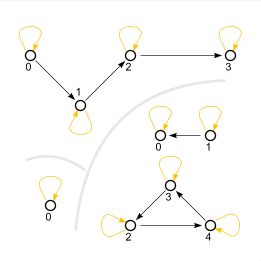
\includegraphics[width=0.27\linewidth]{reflexivgraph} & 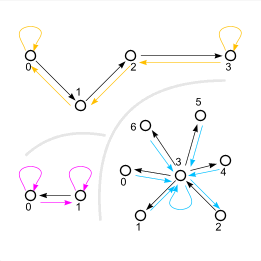
\includegraphics[width=0.27\linewidth]{symmetriegraph} & 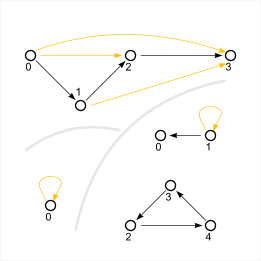
\includegraphics[width=0.27\linewidth]{transitivgraph} \\
				&                                                        & r.u. nicht transi.                                     
			\end{tabular}
		\end{center}
		
		\begin{enumerate}
			\item \textbf{reflexiv} \\\textit{In dieser Abbildung:} Drei reflexive Relationen, als gerichtete Graphen dargestellt.
			
			\item \textbf{symmetrisch} \\\textit{In dieser Abbildung:} Drei symmetrische Relationen, als gerichtete Graphen dargestellt
			
			\item \textbf{transitiv} \\\textit{In dieser Abbildung:} Zwei transitive und eine nicht transitive Relation (rechts unten), als gerichtete Graphen dargestellt.
			
		\end{enumerate}
		
		\subsubsection{Ordnungsrelation}
		\begin{enumerate}
			\item \textbf{reflexiv}
			\item \textbf{transitiv}
			\item \textbf{antisymmetrisch}
		\end{enumerate}
		
		\subsection{Eigenschaften}
		Eine Relation $R \subset A \times A$ hei"st:
		\begin{enumerate}
			\item \textbf{reflexiv}, wenn $(a,a) \in R$ f"ur alle $a \in A$\\Beweisen durch $y := x$
			\item \textbf{symmetrisch}, wenn f"ur alle $(a, b) \in A  \times A$ gilt:\\ $(a,b) \in R \Rightarrow (b,a) \in R$\\Beweisen durch vertauschen von x und y
			\item \textbf{antisymmetrisch}, wenn f"ur alle $a, b \in A$ gilt: \\ $(a, b) \in R$ und $(b, a) \in R \Rightarrow a =b$
			\item \textbf{asymmetrisch},  wenn f"ur alle $a, b \in A$ gilt: \\ $(a, b) \in R \Rightarrow (b, a) \notin R$
			\item \textbf{transitiv},  wenn f"ur alle $a, b, c \in A$ gilt: \\ $(a, b) \in R \land (b,c) \in R \Rightarrow (a, c) \in R$\\Beweisen indem "uber ein anderes Element wieder zum Start gelangt werden kann
		\end{enumerate}
	
		\subsubsection{"Aquivalenzklassen und Beispiel f"ur "Aquivalenzrelation}
		Beispiel"aquivalenzrelation: Auf der Menge A = \{1,2,3,4,5,6\} ist R definiert: $R = \{(a,b) \in A \times A:a^2 \equiv b^2~mod~7\}$
		\begin{enumerate}
			\item Reflexivit"at: $(a, a) \in R.$ Dies gilt da $a^2 \equiv a^2 ~mod~ 7$ gilt.
			\item Symmetrie: $(a, b) \in R \rightarrow (b, a) \in R$. Dies gilt da $a^2 \equiv b^2 ~mod~ 7$ "aquivalent ist zu $b^2 \equiv a^2 ~mod~ 7$ (Gleichheit $~mod~ 7$ ist symmetrisch)
			\item Transitivit"at: analog: Gleichheit $~mod~ 7$ ist transitiv $a^2 \equiv b^2 ~mod~ 7$ und $b^2 \equiv c^2 ~mod~ 7$ folgt $a^2 \equiv c^2 ~mod~ 7$.
		\end{enumerate}
		"Aquivalenzklassen: die Werte von $a^2 ~mod~ 7$ f"ur $a = 1, 2, 3, 4, 5, 6$ sind (alles $~mod~7$):
		$1^2 = 1, 2^2 = 4, 3^2 = 9 = 2, 4^2 = 16 = 2, 5^2 = 25 = 4, 6^2 = 36 = 1$.
		Somit sind die Äquivalenzklassen \{1, 6\}, \{2, 5\} und \{3, 4\}.
		
		\section{Elementare Zahlentheorie}
		\subsection{Quersumme}
		Sei $x \in \mathrm{N}$ und $x = (q_n, q_{n-1}, ... , q_1, q_0 ) =$\\
		$ q_n \cdot 10^n + q_{n-1} \cdot 10^{n-1} + ... + q_1 \cdot 10^1 + q_0 \cdot 10^0$\\ die Dezimaldarstellung von x. Dann gilt:
		
		\begin{enumerate}
			\item \textbf{Quersume:} $Q(x) := q_o + q_1 + ... + q_n$
			\item \textbf{alternierende Quersumme:}\\ $Q'(x) := q_o - q_1 + q_2 ... + (-1)^n \cdot q_n$
			\item $x \equiv Q(x)~mod~9$
			\item $x \equiv Q'(x)~mod~11$
		\end{enumerate}
		
		\subsection{Teilbarkeit}
		\begin{onehalfspacing}
			Sei $d, a \in \mathrm{Z}$ \\
			$d~|~a$ : $d$ teilt $a$ $\Rightarrow$ $r \in \mathrm{Z}$ : $a = d \cdot r$\\
			$d \nmid a$ : $d$ teilt nicht $a$\\
		\end{onehalfspacing}
		\\
		\textbf{Rechenregeln:}
		\begin{enumerate}
			\item $a~|~a$ (reflexiv) 
			\item $(a~|~b) \land (c~|~d) \Rightarrow (a \cdot c)~|~(b \cdot d)$
			\item $a~|~b \land b~|~c \Rightarrow a~|~c$ (transitiv) 
			\item $a~|~b \land a~|~c \Rightarrow a~|~(m \cdot b + n \cdot c)$ f"ur alle $m,n \in \mathrm{Z}$
		\end{enumerate}
		
		\subsection{Primzahlen}
		Eine Zahl $p \in \mathrm{N}$ hei"st Primzahl, wenn:
		\begin{enumerate}
			\item $p > 1$ und
			\item $p = a \cdot b$ mit $a,b \in \mathrm{N}$ $\Rightarrow$ $a =  1 \lor b = 1$\\
			d.h. Primzahlen haben keine echten Teiler
		\end{enumerate}
		
		\subsubsection{Besondere Rechenregeln}
		\begin{onehalfspacing}
			$p~|~(a \cdot b) \Rightarrow p~|~a \lor p~|~b$
		\end{onehalfspacing}
		
		\subsubsection{Hauptsatz der elementaren Zahlentheorie}
		Sei $a \in \mathrm{Z}, a \neq 0$ und $\epsilon = \pm 1$ \\
		\[
		a =  \epsilon \cdot \prod_{p}^{} p^{m_p(a)}
		\]
		\textbf{Beispiel:}\\
		$372 = 2^2 \cdot 3^1 \cdot 31^1$\\
		$m_2(372) = 2, m_3(372) = 1, m_31(372) = 1$
		
		\subsubsection{Anzahl positiver Teiler}
		\[
		\tau(a) =  \prod_{i=1}^{r} (m_i(a)+1)
		\]
		\textbf{Beispiel:}\\
		$120 = 2^3 \cdot 3^1 \cdot 5^1$\\
		$\tau(120) = (3+1)  \cdot (1+1) \cdot (1+1) = 16$
		
		\subsection{Kongruenz}
		\begin{onehalfspacing}
			$a \equiv b~mod~m \Leftrightarrow m | (a - b) \Leftrightarrow (a - b) = m \cdot t \Leftrightarrow a = m \cdot t + b$
		\end{onehalfspacing}
		
		\subsection{ggT, kgV}
		\subsubsection{Gr"o"ster gemeinsamer Teiler}
		Seien $a,b,d \in \mathrm{Z}$ gilt $d = ggT(a,b)$ wenn:
		\begin{enumerate}
			\item $d \geq 0$, $d~|~a~\land~d~|~b$
			\item F"ur jeden gemeinsamen Teiler t von a und b gilt $t~|~a$
		\end{enumerate}
		\textbf{Beispiel:}\\
		$ggT(531, 93) = ggT(3^2 \cdot 59, 3 \cdot 31) = 3$
		\\Taschenrechner: GCD(VAL1;VAL2)
		
		\subsubsection{kleinstes gemeinsames Vielfaches}
		\[
		kgV(a, b) = \frac{|a \cdot b|}{ggT(a,b)}
		\]
		
		\subsection{Diophantische Gleichungen}
		\subsubsection{L"osbarkeit}
		$ax + by = c$ ist l"osbar wenn gilt: $ggT(a,b)~|~c$
		
		\subsubsection{Erweiterter euklidischer Algorithmus}
		Berechnet: $n^{-1}~mod~m$
		\\\textbf{Tabelle Auff"ullen}:
		$r_1 = m,~r_2 = n,~x_1=1,~x_2=0,~y_1=0,~y_2=1$\\
		$\forall~i > 2$ gilt: \\
		$r_{i-2}\verb|:R|r_{i-1} = q_{i-1}\verb|;R=|r_{i}$ (Taschenrechnersyntax)\\
		${x}_i = {x}_{i-2} - (q_{i-1} \cdot  {x}_{i-1} ) $\\
		${y}_i = {y}_{i-2} - (q_{i-1} \cdot  {y}_{i-1} ) $\\
		\\
		\textbf{Beispiel:} $m = 520$ $n = 103$
		\begin{center} 
			\begin{tabular}{ c c c c c }
				i & $r_i$                & $q_i$ & $x_i$                       & $y_i$                       \\
				\hline
				1 & 520                  &       & \colorbox{CarnationPink}{1} & \colorbox{CarnationPink}{0} \\
				2 & 103                  & 5     & \colorbox{CarnationPink}{0} & \colorbox{CarnationPink}{1} \\
				3 & 5                    & 20    & 1                           & -5                          \\
				4 & 3                    & 1     & -20                         & 101                         \\
				5 & 2                    & 1     & 21                          & -106                        \\
				6 & \colorbox{yellow}{1} &       & \colorbox{green}{-41}       & \colorbox{green}{207}       \\
				  &                      &       & \colorbox{SkyBlue}{$=x_0$}  & \colorbox{SkyBlue}{$=y_0$}  \\
			\end{tabular}
		\end{center}
		$ggT(520, 103) = \colorbox{yellow}{1}$ \hfill $103^{-1}~mod~520=\colorbox{green}{207}~(Inverse)$\\
		\\
		$\textbf{Bemerkung:}$ $ggT(m, n) = 1$: so sind $m$ und $n$ \uline{teilerfremd!}\\
		\textbf{Zur Kontrolle:} es muss immer gelten $r_i = r_{i+1} \cdot q_{i+1} + r_{i+2}$
		
		\subsubsection{L"osungsgesamtheit}
		Durch den erweitertern euklidischen Algorithmus erh"alt man eine m"ogliche L"osung der Gleichung $ax + by = c$. Alle ganzzahligen L"osungen erh"alt man wie folgt:
		\[ x = \colorbox{SkyBlue}{$x_0$} + k \cdot \frac{b}{ggT(a,b)}~~~~~~y = \colorbox{SkyBlue}{$y_0$} - k \cdot \frac{a}{ggT(a,b)} \]
		
		\subsubsection{L"osen von Kongruenzgleichungen}
		\begin{align*}
		a \cdot x \equiv b~mod~m 
		\end{align*}
		\textbf{L"osbarkeit:} Die Gleichung ist l"osbar, wenn $ggT(a, m) = 1$\\
		\\
		\textbf{Beispiel:} Gesucht ist ein $x$ mit $103x \equiv 3~mod~520$\\
		\\
		$520x + 103y = 3$\\
		\\
		$520 \cdot 520^{-1} + 103 \cdot 103^{-1} = 1$\\
		$520 \cdot \colorbox{green}{-41} + 103 \cdot \colorbox{green}{207} = 1$$\quad$$| \cdot 3$\\
		$520 \cdot (\colorbox{green}{-41} \cdot 3) + 103 \cdot (\colorbox{green}{207} \cdot 3) = 3$\\
		\\
		$\Rightarrow$ $x=-123$ $y=621$ $\Rightarrow$ $103 \cdot 621 \equiv 3~mod~520$\\
		\\
		\textbf{Hinweis:} Sollte der $ggT(a, m) \neq 1$ sein, sollte gepr"uft werden ob a und b k"urzbar sind.
		
		\subsection{Eulersche $\varphi$-Funktion}
		Sie gibt f"ur jede nat"urliche Zahl $m$ an, wie viele positive ganze Zahlen $a \leq m$ zu ihr tei�lerfremd sind: 
		\[
		\varphi(m) := |\{1 \leq a \leq m~|~ggT(a, m) = 1\}|
		\]
		Sei $\mathrm{Z}^*_m := \{a \in \mathrm{Z}_m~|~a~ist~inventierbar\}$.\\
		Dann gilt: $|\mathrm{Z}^*_m| = \varphi(m) $
		\[
		\varphi(m) = m \prod_{p~|~m}^{} (1 - \frac{1}{p})
		\]
		Ist $p$ eine \uline{Primzahl}, dann gilt:
		\begin{align*}
		\varphi(p)   & = p - 1                                 \\
		\varphi(p^k) & = p^k - p^{k-1} = p^k (1 - \frac{1}{p}) 
		\end{align*}
		\uline{$m$, $n$ teilerfremd:}
		\begin{align*}
		\varphi(m \cdot n) & = \varphi(m) \cdot \varphi(n)                \\
		& \phantom{b=\,}\sum_{d~|~m}^{} \varphi(d) = m 
		\end{align*}
		
		\subsection{Satz von Euler $\&$ der kleine Satz von Fermat}
		\subsubsection{Satz von Euler}
		F"ur $ggT(a, m) = 1$ gilt:
		\[
		a^{\varphi(m)} \equiv 1~mod~m
		\]
		\subsubsection{kleiner Satz von Fermat}
		F"ur $p$ eine Primzahl und $ggT(a, p) = 1$ gilt:
		\[
		a^{p-1}~mod~p \equiv 1~mod~p
		\]
		\subsubsection{Satz von Wilson}
		$(p-1)! \equiv -1(mod~p)$ gilt genau dann, wenn p prim.
		
		\subsubsection{Anwendungsbeispiele}
		\paragraph{Berechnung von $\varphi(2625)$}
		Primfaktorzerlegung: FACT am taschenrechner!\\
		$\varphi(2625) = \varphi(3 \cdot 5^3 \cdot 7) = (3^1-3^0)(5^3-5^2)(7^1-7^0) = 1200$ 
		\paragraph{Berechnung von $13^{6005}~mod~2625$ - Satz von Euler}
		\begin{onehalfspacing}
			$ggT(13, 2625) = 1$\\
			$13^{1200} \equiv 1~mod~2625$\\
			\\
			$13^{6005}~mod~2625 = 13^{1200 \cdot 5 + 5} = (13^{1200})^5 \cdot 13^{5} \equiv \\
			1^5 \cdot 13^5~mod~2625 = 13^5~mod~2625 = 371293 = 1168~mod~2625$
		\end{onehalfspacing}
		\paragraph{Berechnung von $6005^{(\varphi(6005))}~mod~13$ - Kleiner Satz von Fermat}
		\begin{onehalfspacing}
			$6005^{(\varphi(6005))}~mod~13 \equiv 12^{(\varphi(6005))} \equiv 12^{1200} \equiv 12^{(12 \cdot 100)} \equiv (12^{12})^{100} \equiv 1^{100} \equiv 1~mod~13$
		\end{onehalfspacing}
		\subsection{Modulares Potenzieren}
		\subsubsection{Regel I}L"asst sich der Exponent als Summe zweier kleinerer Zahlen darstellen, so gilt:\\\\
		$x^{a+b} = x^a \cdot x^b$\\\\
		Soll der Rest der Potenz gebildet werden, so kann die Restfunktion bereits auf Zwischenergebnisse angewendet werden, denn bez"uglich der Restbildung zur Division durch d gilt:
		\\\\
		$x^{a+b}~mod~d = ((x^a~mod~d) \cdot (x^b~mod~d))~mod~d $
		\subsubsection{Regel II}
		L"asst sich der Exponent als Produkt zweier kleinerer Zahlen darstellen, so gilt:\\\\
		$x^{a\cdot b} = (x^a)^b$\\\\
		Soll der Rest der Potenz gebildet werden, so kann die Restfunktion bereits auf Zwischenergebnisse angewendet werden, denn bez"uglich der Restbildung zur Division durch d gilt:\\\\
		$x^{a\cdot b}~mod~d = (x^a~mod~d)^b~mod~d$
		\subsubsection{Anwendung und Sonderf"alle}
		$(a-1)^{gerade~zahl}~mod~a \equiv (-1)^{gerade}~mod~a  \equiv 1$\\
		$(a-1)^{ungerade~zahl}~mod~a \equiv (-1)^{ungerade}~mod~a  \equiv -1$\\
		$a^{n}~mod~a+1 \equiv 1^n~mod~a \equiv 1$\\
		
		\subsection{Chinesischer Restsatz}
		\begin{align*}
		x \equiv a_1~mod~m_1 \\
		x \equiv a_2~mod~m_2 \\
		x \equiv a_3~mod~m_3 
		\end{align*}
		
		\subsubsection{L"osbarkeit}
		$ggT(m_1, m_2, m_3) = 1$ $\Rightarrow$ eindeutig l"osbar;
		sonst hat das System 0 oder mehrere L"osungen
		\begin{minipage}{\linewidth}
			\subsubsection{Konstruktive L"osung}
			
			\begin{onehalfspacing}
				\boxed{$$x \equiv \colorbox{yellow}{r}~mod~\colorbox{green}{$q_{i}$}$~~$m_i = \colorbox{green}{$q_{i+1}$}      \cdot \colorbox{green}{$q_{i+2}$} = \colorbox{CornflowerBlue}{$m_{i}$}$$}\\
				$x \equiv \colorbox{yellow}{4}~mod~\colorbox{green}{20}$~~$m_1 = \colorbox{green}{21}      \cdot \colorbox{green}{23} = \colorbox{CornflowerBlue}{483}$\\
				$x \equiv \colorbox{yellow}{5}~mod~\colorbox{green}{21}$~~$m_2 = \colorbox{green}{20} \cdot \colorbox{green}{23} = \colorbox{CornflowerBlue}{460}$  \\
				$x \equiv \colorbox{yellow}{6}~mod~\colorbox{green}{23}$~~$m_2 = \colorbox{green}{20} \cdot \colorbox{green}{21} = \colorbox{CornflowerBlue}{420}$  \\
				\\
				\boxed{$$m = \colorbox{green}{$q_1$} \cdot \colorbox{green}{$q_2$} \cdot \colorbox{green}{$q_3$} = \colorbox{Melon}{m}$$}\\
				$m = \colorbox{green}{20} \cdot \colorbox{green}{21} \cdot \colorbox{green}{23} = \colorbox{Melon}{9660}$\\
				\\
				$M_i$ so w"ahlen, dass $(r_i \cdot M_i)~mod~m_i \equiv 1$\\
				Wenn $M_i$ nicht sofort ersichtlich, dann Euklid anwenden mit den Startwerten: $(\colorbox{CornflowerBlue}{$m_i$}~mod~\colorbox{green}{$q_i$})^{-1}~mod~\colorbox{green}{$q_i$}$
				\boxed{$$M_i: \colorbox{CornflowerBlue}{$ m_i~$} \cdot M_i~mod~\colorbox{green}{$q_i$} \equiv ((\colorbox{CornflowerBlue}{$m_i$}\%\colorbox{green}{$q_i$})\cdot \colorbox{CarnationPink}{$M_1$})\%\colorbox{green}{$q_i$} \equiv 1\%q_i$$}\\
				$M_1: \colorbox{CornflowerBlue}{483} \cdot M_1~mod~\colorbox{green}{20} \equiv (3~\cdot \colorbox{CarnationPink}{$M_1$})~mod~\colorbox{green}{20} \equiv 1~mod~20$\\
				$M_2: \colorbox{CornflowerBlue}{460} \cdot M_2~mod~\colorbox{green}{21} \equiv (19\cdot \colorbox{CarnationPink}{$M_2$})~mod~\colorbox{green}{21} \equiv 1~mod~21$\\
				$M_3: \colorbox{CornflowerBlue}{420} \cdot M_3~mod~\colorbox{green}{23} \equiv (6~\cdot \colorbox{CarnationPink}{$M_3$})~mod~\colorbox{green}{23} \equiv 1~mod~23$\\
				\\
				\boxed{$$x \equiv (\colorbox{yellow}{$r_1$}\colorbox{CornflowerBlue}{$m_1$}\colorbox{CarnationPink}{$M_1$} + \colorbox{yellow}{$r_2$}\colorbox{CornflowerBlue}{$m_2$}\colorbox{CarnationPink}{$M_2$} + \colorbox{yellow}{$r_3$}\colorbox{CornflowerBlue}{$m_3$}\colorbox{CarnationPink}{$M_3$})~mod~\colorbox{Melon}{m}$$}\\
				$\colorbox{yellow}{4} \cdot \colorbox{CornflowerBlue}{483} \cdot  \colorbox{CarnationPink}{7} + \colorbox{yellow}{5} \cdot \colorbox{CornflowerBlue}{460} \cdot  \colorbox{CarnationPink}{10} + \colorbox{yellow}{6} \cdot \colorbox{CornflowerBlue}{420} \cdot  \colorbox{CarnationPink}{4} = 46604~mod~\colorbox{Melon}{9660}$\\
				\\
				$x \equiv 7964~mod~\colorbox{Melon}{9660}$
			\end{onehalfspacing}
		\end{minipage}
		
		\section{Kombinatorik}
		\subsection{Binomialkoeffizienten}
		F"ur $n,k \in \mathrm{R}$, $0 \leq k \leq n$:\\
		\[ \binom{n}{k} =  \frac{n!}{k! \cdot (n-k)!}  \] 
		Symmetrie im pascalschen Dreieck:\\
		\[ \binom{n}{k} =  \binom{n}{n-k}  \] 
		Rekursive Definition:\\
		\[ \binom{n}{k} =  \binom{n-1}{k-1} + \binom{n-1}{k} \] 
		Binomischer Lehrsatz:\\
		\[ (a+b)^n =  \sum_{k=0}^{n} \binom{n}{k} a^{n-k} \cdot b^k \] 
		\subsection{Stichproben}
		$M := $ Menge von Objekten die entweder die Eigenschaft $A$ oder $B$ haben.
		
		$M = A \cup B, \; A \cap B = \varnothing$
		
		$|A|$ Elementen haben die Eigenschaft $A$.
		
		Stichprobe enth"alt $x$ Elementen
		
		\uline{Anzahl der m"oglichen Stichproben} jenach Anzahl der Elementen 
		aus $A$ die eine Stichprobe
		mit insgesamt $x$ Elementen enth"alt:
		\subsubsection{Mindestens eins aus A}
		= Alle - keines aus A 
		\subsubsection{Kein Element aus A}
		\[ \binom{|B|}{x} \]
		
		\subsubsection{Genau y Elementen aus A}
		\[
		\binom{|A|}{y} \cdot \binom{|B|}{x - y} 
		\]
		
		\subsubsection{H"ochstens y Elementen aus A}
		\[
		\sum_{i = 0}^{y} \binom{|A|}{i} \cdot \binom{|B|}{x - i}
		\]
		
		\subsubsection{Mindestens y Elementen aus A}
		\begin{align*}
		& \sum_{i = y}^{|A|} \binom{|A|}{i} \cdot \binom{|B|}{x - i} 
		\end{align*}
		
		\subsection{Zusammenfassung}
		\begin{tabular}{p{2.65cm} | p{2.65cm} | p{2.65cm}}
			Auswahl...                                                 & \textbf{ohne} Beachtung der Reihenfolge (Kombination) $(b,a) = (a,b)$ & \textbf{mit} Beachtung der Reihenfolge (Variation) $(a,b) \neq (b,a)$ \\
			\hline
			\textbf{ohne} Zur"ucklegen (Element wiederholt sich nicht) & \[ \binom{n}{k} \] Taschenrechner: $n$C$r \rightarrow n$C$k$          & \[ \frac{n!}{(n-k)!} \] Taschenrechner: $n$P$r \rightarrow n$P$k$     \\
			\hline
			\textbf{mit} Zur"ucklegen (Element wiederholt sich)        & \[ \binom{n + k -1}{k} \]                                             & \[ n^k \]                                                             \\
		\end{tabular}
		\paragraph{Beispiele}
		\noindent\begin{tabular}{p{2.65cm} | p{2.65cm} | p{2.2cm}}
			& & Reihenfolge    \\
			\hline
			Permutation ohne Wiederholung & $n!$ & beachten       \\
			\hline
			Permutation mit Wiederholung  & $\frac{n!}{k_1! \cdot  k_2! \cdot \text{...} \cdot k_s!}$ & beachten       \\
			\hline
			Variation ohne Wiederholung   & $\frac{n!}{(n-k)!}$ & beachten       \\
			\hline
			Variation mit Wiederholung    & $n^k$ & beachten       \\
			\hline
			Kombination ohne Wiederholung & ${n \choose k}$ & nicht beachten \\
			\hline
			Kombination mit Wiederholung  & ${n+k-1 \choose k}$ & nicht beachten \\
		\end{tabular}
		\\
		
		Sind die \textbf{Objekte untereinander unterscheidbar}, so spricht man von einer Permutation/Variation/Kombination "ohne Wiederholung" (derselben Objekte). Falls die Objekte jedoch \textbf{nicht unterscheidbar} sind, spricht man von einer Permutation/Variation/Kombination "mit Wiederholung". Im Urnenmodell sagt man statt "ohne Wiederholung" einfach "ohne Zur"ucklegen" und zu "mit Wiederholung" entsprechend "mit Zur"ucklegen".
		
		\subsection{Das Schubfachprinzip}
		Falls man $n$ Objekte auf $m$ Mengen ($n, m > 0$) verteilt und $n$ gr"o"ser als $m$ ist, dann gibt es mindestens eine Menge, in der mehr als ein Objekt landet.
		
		\subsection{Das Inklusions-Exklusionsprinzip}
		F"ur die Mengen $A$, $B$, $C$ und $A_i$ gilt:
		\begin{enumerate}
			\item $| A \cup B | = |A| + |B| - |A \cap B |$
			\item $| A \cup B \cup C | = |A| + |B| + |C| - |A \cap B | - |A \cap C |\\- |B \cap C | + |A \cap B \cap C | $
			\item Allgemein: $| A_1 \cup A_2 \cup ... \cup A_n | = |A_1| + ... + |A_n|\\-  |A_1 \cap A_2 | - ... + (-1)^{n-1} \cdot  |A_1 \cap ... \cap A_n | $
		\end{enumerate}

		\subsubsection{Beispiel}
			Wie viele Zahlen 1, ..., 1000 sind durch 2,3 oder 5 teilbar?
			$N = \floor*{\frac{1000}{2}} + \floor*{\frac{1000}{3}} + \floor*{\frac{1000}{5}} - \floor*{\frac{1000}{2 \cdot 3}} - \floor*{\frac{1000}{2 \cdot 5}} - \floor*{\frac{1000}{3 \cdot 5}} + \floor*{\frac{1000}{2 \cdot 3 \cdot 5}}$
		
		
		\section{Komplexe Zahlen}
		\subsection{Darstellung}
		\subsubsection{Kartesische Darstellung}
		$(x, y)$ kartesische Koordinaten\\
		\[ z = x +iy \]
		\[
		Re(z) =  \frac{z + \overline{z}}{2} ~~~~~~ Im(z) = \frac{z - \overline{z}}{2i}
		\]
		
		\subsubsection{Polare Darstellung}
		$(r, \varphi)$ Polarkoordinaten\\
		$r = |z|$ Betrag\\
		$\varphi$ Winkel zur x-Achse ($-\pi < \varphi \leq \pi $) 
		\[ z = r \cdot (cos(\varphi) + i \cdot sin(\varphi))\]
		\[ \mathrm{e}^{i\varphi} = cos(\varphi) + i \cdot sin(\varphi) ~~~ (Euler)\]
		
		\[ z = r \cdot \mathrm{e}^{i\varphi} ~~~ (Polardarstellung) \]
		
		\textbf{Sonderfall}: $-1 = e^{i\pi}$
		
		\subsubsection{Umrechnungen}
		\paragraph{Kartesische in Polare Darstellung}
		Umrechnung von $z = x + i \cdot y \in \mathrm{C}$ zu  $z =  r \cdot \mathrm{e}^{i\varphi} \in \mathrm{C}$:
		\[ r = \sqrt{x^2 +y^2} \]
		\[ \varphi = \begin{cases} arccos(\frac{x}{r}) &\mbox{if } y \geq 0 \\ 
		- arccos(\frac{x}{r}) &\mbox{if } y < 0 \end{cases} \]
		
		\paragraph{Polare in Kartesische Darstellung}
		Umrechnung von $z =  r \cdot \mathrm{e}^{i\varphi} \in \mathrm{C}$ zu $z = x + i \cdot y \in \mathrm{C}$:
		\[ z = r \cdot (cos(\varphi) + i \cdot sin(\varphi))\]
		\subsubsection{Konjugiert komplexe Zahl}
		\begin{align*}
		\overline{z} & = x - iy                              \\
		& = cos(\varphi) - i \cdot sin(\varphi) \\
		& = \mathrm{e}^{-i\varphi}              
		\end{align*}
		\subsection{Rechenregeln}
		\subsubsection{Addition $\&$ Subtraktion}
		\begin{align*}
		z_1 + z_2 = (x_1 + x_2) + i (y_1 +y_2) \\
		z_1 - z_2 = (x_1 - x_2) + i (y_1 -y_2) 
		\end{align*}
		\subsubsection{Multiplikation}
		\begin{align*}
		z_1 \cdot z_2                                               & = (x_1x_2 - y_1y_2) + i (x_1y_2 + x_2y_1)     \\
		r_1\mathrm{e}^{i\varphi_1} \cdot r_2\mathrm{e}^{i\varphi_2} & = r_1r_2\mathrm{e}^{i(\varphi_1 + \varphi_2)} 
		\end{align*}
		Betr"age multiplizieren und Winkel addieren
		\subsubsection{Potenzieren}
		\begin{align*}
		z^n = (r \cdot \mathrm{e}^{i\varphi})^n =  r^n \cdot \mathrm{e}^{i \cdot n\varphi} 
		\end{align*}
		Betrag mit $n$ potenzieren, Winkel mit $n$ multiplizieren
		\subsubsection{Division}
		\begin{align*}
		\frac{x_1 + i \cdot y_1}{x_2 + i \cdot y_2}                   & = \frac{(x_1 + i \cdot y_1)(x_2 - i \cdot y_2)}{(x_2 + i \cdot y_2)(x_2 - i \cdot y_2)} =           \\
		& = \frac{(x_1x_2 + y_1y_2)}{({x_2}^2 + {y_2}^2)} + \frac{ i (x_1y_2 + x_2y_1) }{({x_2}^2 + {y_2}^2)} \\
		\frac{r_1\mathrm{e}^{i\varphi_1}}{r_2\mathrm{e}^{i\varphi_2}} & = \frac{r_1}{r_2}\mathrm{e}^{i(\varphi_1-\varphi_2)}                                                
		\end{align*}
		Betr"age dividieren und Winkel subtrahieren
		\subsubsection{Wurzelziehen}
		\[ \sqrt{z} = \sqrt{r \cdot \mathrm{e}^{i\varphi}} = \pm \sqrt{r} \cdot \mathrm{e}^{i \frac{\varphi}{2}} \]
		Wurzel aus Betrag, halber Winkel.\\
		Allgemein f"ur $k \in {0, 1, 2, ..., n-1}$:
		\begin{align*}
		\sqrt[n]{z} & = \sqrt[n]{r \cdot \mathrm{e}^{i\varphi}}                                                                   \\
		& = \sqrt[n]{r} \cdot e^{i \frac{\varphi + k \cdot 2\pi}{n}}                                                  \\
		& = \sqrt[n]{r} \cdot e^{i (\frac{\varphi}{n} + \frac{k \cdot 2\pi}{n})}                                      \\
		& = \sqrt[n]{r} \cdot (cos(\frac{\varphi + k \cdot 2\pi}{n}) + i \cdot sin(\frac{\varphi + k \cdot 2\pi}{n})) 
		\end{align*}
		
		\subsubsection{Betrag}
		\[ |z| = \sqrt{x^2 + y^2} = \sqrt{z \cdot \overline{z}}  \]
		
		\subsubsection{Weitere wichtige Zusammenh"ange}
		\[ i^{-1} = \frac{1}{i} = -i \]
		\[ i^0 = 1, i^1 = i, i^2 = -1, i^3 = -i, i^4 = 1, i^5 = i, i^6 = -1, i^7 = -i  \]
		\[ (x-(a+ib))(x-(a-ib)) = x^2-2ax+a^2+b^2 \]
		
		\subsection{Quadratische Gleichungen}
		\[ ax^2 +bx + c = 0 \]
		\[ x_{1,2} = \frac{-b \pm \sqrt{b^2 -4ac}}{2a} \]
		\uline{Diskriminante:} $D = b^2 -4ac$\\
		\\
		L"osungen:
		\begin{enumerate}
			\item $D > 0$ $\Rightarrow$ 2 verschiedene reelle L"osungen: \\
			\[ x_{1,2} = \frac{-b \pm \sqrt{D}}{2a} \]
			\item $D = 0$ $\Rightarrow$ 1 doppelte reelle L"osungen:
			\[ x_{1,2} = \frac{-b}{2a} \]
			\item $D < 0$ $\Rightarrow$ 2 konjugiert komplexe L"osungen:
			\[ x_{1,2} = \frac{-b \pm \sqrt{-D}}{2a} \]
		\end{enumerate}
		
		\subsection{Anwendungsbeispiele}
		\subsubsection{1. Variante}
		Die Funktion $f(x) = a_4x^4 +  a_3x^3 +  a_2x^2 +  a_1x +  a_0$ hat die Nullstellen $x_1 = i$ und $x_2 = -1 - i$ gesucht $a_4, ... , a_0 \in \mathrm{R}$\\
		\\
		$x_3 = -i$, $x_4 = -1 + i$ \\
		\\
		$f(x) = (x-i)(x-(-1-i))(x+i)(x-(-1+i)) = ...$\\
		$= (x^2 +1)(x^2 +2x + 2) = ... = (x^4 + 2x^3 + 3x^2 + 2x + 2)$\\
		\\
		$a_4 = 1$, $a_3 = 2$, $a_2 = 3$, $a_1 = 2$, $a_0 = 2$ 
		\subsubsection{2. Variante}
		Die Funktion $f(x) = x^5 - 5x^4 + 12x^3 - 12x^2 -5x +25$ hat die Nullstellen $x_1 = 1 - 2i$ und $x_2 = -1$ gesucht sind alle Nullstellen.\\
		\\
		$x_3 = 1 + 2i$, $x_4 = ?$, $x_5 = ?$ \\
		\\
		Polynomdivision:\\
		$(x^5 - 5x^4 + 12x^3 - 12x^2 -5x +25) : (x +1)$\\$= x^4-6x^3+ 18x^2 -30x +25$\\
		\\
		$(x-(1-2i))(x-(1+2i)) = (x-1+2i)(x-1-2i) = x^2-2x+1-4i^2 = x^2-2x+5 $\\
		\\
		Polynomdivision:\\
		$( x^4-6x^3+ 18x^2 -30x +25) : (x^2-2x+5)$\\$= x^2-4x+5$\\
		\\
		Nullstellen von $x^2-4x+5$:\\
		\[ x_{1,2} = \frac{4 \pm \sqrt{-4}}{2} = \frac{4 \pm 2i}{2} = 2 \pm i \]
		\\
		reelle Faktorisierung:\\
		$f(x) = (x+1)(x^2-2x+5)(x^2-2x+5)(x^2-4x+5)$\\
		\\
		komplexe Faktorisierung:\\
		$f(x) =(x+1)(x-1+2i)(x-1-2i)(x-2-i)(x-2+i)$\\
		
		
	\end{multicols*}
\end{document}